
%% bare_conf_compsoc.tex
%% V1.4b
%% 2015/08/26
%% by Michael Shell
%% See:
%% http://www.michaelshell.org/
%% for current contact information.
%%
%% This is a skeleton file demonstrating the use of IEEEtran.cls
%% (requires IEEEtran.cls version 1.8b or later) with an IEEE Computer
%% Society conference paper.
%%
%% Support sites:
%% http://www.michaelshell.org/tex/ieeetran/
%% http://www.ctan.org/pkg/ieeetran
%% and
%% http://www.ieee.org/

%%*************************************************************************
%% Legal Notice:
%% This code is offered as-is without any warranty either expressed or
%% implied; without even the implied warranty of MERCHANTABILITY or
%% FITNESS FOR A PARTICULAR PURPOSE!
%% User assumes all risk.
%% In no event shall the IEEE or any contributor to this code be liable for
%% any damages or losses, including, but not limited to, incidental,
%% consequential, or any other damages, resulting from the use or misuse
%% of any information contained here.
%%
%% All comments are the opinions of their respective authors and are not
%% necessarily endorsed by the IEEE.
%%
%% This work is distributed under the LaTeX Project Public License (LPPL)
%% ( http://www.latex-project.org/ ) version 1.3, and may be freely used,
%% distributed and modified. A copy of the LPPL, version 1.3, is included
%% in the base LaTeX documentation of all distributions of LaTeX released
%% 2003/12/01 or later.
%% Retain all contribution notices and credits.
%% ** Modified files should be clearly indicated as such, including  **
%% ** renaming them and changing author support contact information. **
%%*************************************************************************


% *** Authors should verify (and, if needed, correct) their LaTeX system  ***
% *** with the testflow diagnostic prior to trusting their LaTeX platform ***
% *** with production work. The IEEE's font choices and paper sizes can   ***
% *** trigger bugs that do not appear when using other class files.       ***                          ***
% The testflow support page is at:
% http://www.michaelshell.org/tex/testflow/



\documentclass[conference,compsoc,fleqn]{IEEEtran}
\usepackage[utf8]{inputenc}
\usepackage{amsmath}
\usepackage{latexsym}
\usepackage{graphicx}
\usepackage{color}
\usepackage{geometry}
\usepackage{empheq}
\usepackage{tikz}
\usepackage{pgfplots}
\usepackage{amsfonts}
\usepackage{commath}
\usepackage{gensymb}
\usepackage{float}
\usepackage{multirow}
\usepackage{hyperref}
\usepackage{indentfirst}
\usepackage{empheq}
%\usepackage{mathptmx}
\usepackage{amssymb}
\usepackage{cancel}
\usepackage{bm}
\usepackage{siunitx}
\usepackage{tcolorbox}
\usepackage{filecontents}
\usepackage[numbers, sort&compress]{natbib}
\usepackage{setspace}
\usepackage[font=small, labelfont=bf]{caption}
\usepackage{enumerate}
\usepackage{nccmath}
\usepackage{booktabs}
\usepackage{wasysym}
\usepackage{xcolor}
\usepackage{fancyhdr}
\usepackage{lastpage}
\usetikzlibrary{shapes.geometric,calc}
\pgfplotsset{compat=1.4}
% \addtolength{\oddsidemargin}{-.875in}
% \addtolength{\evensidemargin}{-.875in}
% \addtolength{\textwidth}{1.75in}
% 
% \addtolength{\topmargin}{-.875in}
% \addtolength{\textheight}{1.75in}
\pgfplotsset{compat=newest} % Allows to place the legend below plot
\usepgfplotslibrary{units} % Allows to enter the units nicely
% Some/most Computer Society conferences require the compsoc mode option,
% but others may want the standard conference format.
%
% If IEEEtran.cls has not been installed into the LaTeX system files,
% manually specify the path to it like:
% \documentclass[conference,compsoc]{../sty/IEEEtran}
%\setlength\extrarowheight{3pt}





% Some very useful LaTeX packages include:
% (uncomment the ones you want to load)


% *** MISC UTILITY PACKAGES ***
%
%\usepackage{ifpdf}
% Heiko Oberdiek's ifpdf.sty is very useful if you need conditional
% compilation based on whether the output is pdf or dvi.
% usage:
% \ifpdf
%   % pdf code
% \else
%   % dvi code
% \fi
% The latest version of ifpdf.sty can be obtained from:
% http://www.ctan.org/pkg/ifpdf
% Also, note that IEEEtran.cls V1.7 and later provides a builtin
% \ifCLASSINFOpdf conditional that works the same way.
% When switching from latex to pdflatex and vice-versa, the compiler may
% have to be run twice to clear warning/error messages.






% *** CITATION PACKAGES ***
%
%\ifCLASSOPTIONcompsoc
  % IEEE Computer Society needs nocompress option
  % requires cite.sty v4.0 or later (November 2003)
  %\usepackage[nocompress]{cite}
%\else
  % normal IEEE
  %\usepackage{cite}
%\fi
% cite.sty was written by Donald Arseneau
% V1.6 and later of IEEEtran pre-defines the format of the cite.sty package
% \cite{} output to follow that of the IEEE. Loading the cite package will
% result in citation numbers being automatically sorted and properly
% "compressed/ranged". e.g., [1], [9], [2], [7], [5], [6] without using
% cite.sty will become [1], [2], [5]--[7], [9] using cite.sty. cite.sty's
% \cite will automatically add leading space, if needed. Use cite.sty's
% noadjust option (cite.sty V3.8 and later) if you want to turn this off
% such as if a citation ever needs to be enclosed in parenthesis.
% cite.sty is already installed on most LaTeX systems. Be sure and use
% version 5.0 (2009-03-20) and later if using hyperref.sty.
% The latest version can be obtained at:
% http://www.ctan.org/pkg/cite
% The documentation is contained in the cite.sty file itself.
%
% Note that some packages require special options to format as the Computer
% Society requires. In particular, Computer Society  papers do not use
% compressed citation ranges as is done in typical IEEE papers
% (e.g., [1]-[4]). Instead, they list every citation separately in order
% (e.g., [1], [2], [3], [4]). To get the latter we need to load the cite
% package with the nocompress option which is supported by cite.sty v4.0
% and later.





% *** GRAPHICS RELATED PACKAGES ***
%
\ifCLASSINFOpdf
  % \usepackage[pdftex]{graphicx}
  % declare the path(s) where your graphic files are
  % \graphicspath{{../pdf/}{../jpeg/}}
  % and their extensions so you won't have to specify these with
  % every instance of \includegraphics
  % \DeclareGraphicsExtensions{.pdf,.jpeg,.png}
\else
  % or other class option (dvipsone, dvipdf, if not using dvips). graphicx
  % will default to the driver specified in the system graphics.cfg if no
  % driver is specified.
  % \usepackage[dvips]{graphicx}
  % declare the path(s) where your graphic files are
  % \graphicspath{{../eps/}}
  % and their extensions so you won't have to specify these with
  % every instance of \includegraphics
  % \DeclareGraphicsExtensions{.eps}
\fi
% graphicx was written by David Carlisle and Sebastian Rahtz. It is
% required if you want graphics, photos, etc. graphicx.sty is already
% installed on most LaTeX systems. The latest version and documentation
% can be obtained at:
% http://www.ctan.org/pkg/graphicx
% Another good source of documentation is "Using Imported Graphics in
% LaTeX2e" by Keith Reckdahl which can be found at:
% http://www.ctan.org/pkg/epslatex
%
% latex, and pdflatex in dvi mode, support graphics in encapsulated
% postscript (.eps) format. pdflatex in pdf mode supports graphics
% in .pdf, .jpeg, .png and .mps (metapost) formats. Users should ensure
% that all non-photo figures use a vector format (.eps, .pdf, .mps) and
% not a bitmapped formats (.jpeg, .png). The IEEE frowns on bitmapped formats
% which can result in "jaggedy"/blurry rendering of lines and letters as
% well as large increases in file sizes.
%
% You can find documentation about the pdfTeX application at:
% http://www.tug.org/applications/pdftex





% *** MATH PACKAGES ***
%
%\usepackage{amsmath}
% A popular package from the American Mathematical Society that provides
% many useful and powerful commands for dealing with mathematics.
%
% Note that the amsmath package sets \interdisplaylinepenalty to 10000
% thus preventing page breaks from occurring within multiline equations. Use:
%\interdisplaylinepenalty=2500
% after loading amsmath to restore such page breaks as IEEEtran.cls normally
% does. amsmath.sty is already installed on most LaTeX systems. The latest
% version and documentation can be obtained at:
% http://www.ctan.org/pkg/amsmath





% *** SPECIALIZED LIST PACKAGES ***
%
%\usepackage{algorithmic}
% algorithmic.sty was written by Peter Williams and Rogerio Brito.
% This package provides an algorithmic environment fo describing algorithms.
% You can use the algorithmic environment in-text or within a figure
% environment to provide for a floating algorithm. Do NOT use the algorithm
% floating environment provided by algorithm.sty (by the same authors) or
% algorithm2e.sty (by Christophe Fiorio) as the IEEE does not use dedicated
% algorithm float types and packages that provide these will not provide
% correct IEEE style captions. The latest version and documentation of
% algorithmic.sty can be obtained at:
% http://www.ctan.org/pkg/algorithms
% Also of interest may be the (relatively newer and more customizable)
% algorithmicx.sty package by Szasz Janos:
% http://www.ctan.org/pkg/algorithmicx




% *** ALIGNMENT PACKAGES ***
%
%\usepackage{array}
% Frank Mittelbach's and David Carlisle's array.sty patches and improves
% the standard LaTeX2e array and tabular environments to provide better
% appearance and additional user controls. As the default LaTeX2e table
% generation code is lacking to the point of almost being broken with
% respect to the quality of the end results, all users are strongly
% advised to use an enhanced (at the very least that provided by array.sty)
% set of table tools. array.sty is already installed on most systems. The
% latest version and documentation can be obtained at:
% http://www.ctan.org/pkg/array


% IEEEtran contains the IEEEeqnarray family of commands that can be used to
% generate multiline equations as well as matrices, tables, etc., of high
% quality.




% *** SUBFIGURE PACKAGES ***
%\ifCLASSOPTIONcompsoc
%  \usepackage[caption=false,font=footnotesize,labelfont=sf,textfont=sf]{subfig}
%\else
%  \usepackage[caption=false,font=footnotesize]{subfig}
%\fi
% subfig.sty, written by Steven Douglas Cochran, is the modern replacement
% for subfigure.sty, the latter of which is no longer maintained and is
% incompatible with some LaTeX packages including fixltx2e. However,
% subfig.sty requires and automatically loads Axel Sommerfeldt's caption.sty
% which will override IEEEtran.cls' handling of captions and this will result
% in non-IEEE style figure/table captions. To prevent this problem, be sure
% and invoke subfig.sty's "caption=false" package option (available since
% subfig.sty version 1.3, 2005/06/28) as this is will preserve IEEEtran.cls
% handling of captions.
% Note that the Computer Society format requires a sans serif font rather
% than the serif font used in traditional IEEE formatting and thus the need
% to invoke different subfig.sty package options depending on whether
% compsoc mode has been enabled.
%
% The latest version and documentation of subfig.sty can be obtained at:
% http://www.ctan.org/pkg/subfig




% *** FLOAT PACKAGES ***
%
%\usepackage{fixltx2e}
% fixltx2e, the successor to the earlier fix2col.sty, was written by
% Frank Mittelbach and David Carlisle. This package corrects a few problems
% in the LaTeX2e kernel, the most notable of which is that in current
% LaTeX2e releases, the ordering of single and double column floats is not
% guaranteed to be preserved. Thus, an unpatched LaTeX2e can allow a
% single column figure to be placed prior to an earlier double column
% figure.
% Be aware that LaTeX2e kernels dated 2015 and later have fixltx2e.sty's
% corrections already built into the system in which case a warning will
% be issued if an attempt is made to load fixltx2e.sty as it is no longer
% needed.
% The latest version and documentation can be found at:
% http://www.ctan.org/pkg/fixltx2e


%\usepackage{stfloats}
% stfloats.sty was written by Sigitas Tolusis. This package gives LaTeX2e
% the ability to do double column floats at the bottom of the page as well
% as the top. (e.g., "\begin{figure*}[!b]" is not normally possible in
% LaTeX2e). It also provides a command:
%\fnbelowfloat
% to enable the placement of footnotes below bottom floats (the standard
% LaTeX2e kernel puts them above bottom floats). This is an invasive package
% which rewrites many portions of the LaTeX2e float routines. It may not work
% with other packages that modify the LaTeX2e float routines. The latest
% version and documentation can be obtained at:
% http://www.ctan.org/pkg/stfloats
% Do not use the stfloats baselinefloat ability as the IEEE does not allow
% \baselineskip to stretch. Authors submitting work to the IEEE should note
% that the IEEE rarely uses double column equations and that authors should try
% to avoid such use. Do not be tempted to use the cuted.sty or midfloat.sty
% packages (also by Sigitas Tolusis) as the IEEE does not format its papers in
% such ways.
% Do not attempt to use stfloats with fixltx2e as they are incompatible.
% Instead, use Morten Hogholm'a dblfloatfix which combines the features
% of both fixltx2e and stfloats:
%
% \usepackage{dblfloatfix}
% The latest version can be found at:
% http://www.ctan.org/pkg/dblfloatfix




% *** PDF, URL AND HYPERLINK PACKAGES ***
%
%\usepackage{url}
% url.sty was written by Donald Arseneau. It provides better support for
% handling and breaking URLs. url.sty is already installed on most LaTeX
% systems. The latest version and documentation can be obtained at:
% http://www.ctan.org/pkg/url
% Basically, \url{my_url_here}.




% *** Do not adjust lengths that control margins, column widths, etc. ***
% *** Do not use packages that alter fonts (such as pslatex).         ***
% There should be no need to do such things with IEEEtran.cls V1.6 and later.
% (Unless specifically asked to do so by the journal or conference you plan
% to submit to, of course. )


% correct bad hyphenation here
\hyphenation{op-tical net-works semi-conduc-tor}
\geometry{left=2.03cm,right=2.03cm,top=2.95cm,bottom=2.03cm}

\newcommand{\graficoctc}[4]{%
	\centering
	%\begin{minipage}[t][6cm][c]{4.5cm}				
		\begin{tikzpicture}[scale=0.81]
		\begin{axis}[
		axis lines=left,
		%/pgf/number format/1000 sep={.},/pgf/number format/use comma,
		%		xmin = 0,
		%		xmax = 0.04,
		%		ymin = 310,
		%		ymax = 340,
		%		restrict y to domain=-500:2000,
		scaled x ticks = false,
		scaled y ticks = false,
		x tick label style={/pgf/number format/fixed},
		y tick label style={/pgf/number format/fixed},
		anchor=east,  
		width=6cm,
		height=5cm,
		label style={font=\footnotesize},
		xlabel = $x$(m),
		xlabel style={at={(1.2, 0)}, anchor = east},
		ylabel= $h_c$ (W/$\text{m}^2$\celsius),		
		ylabel style={rotate=-90, at={(-0.1, 1)}, anchor = south west}]
		\pgfplotstableread{../data/conductance_#2.dat} 
		\teff
		\addplot[color=black, line width=1.5pt] table from \teff;
		\pgfplotstableread{../data/estimativa_ctc_interface_#1_conductance_#2_stdev_00.dat} 
		\teff
		\addplot[only marks, color=blue,mark=o,mark options={mark size=1.5pt}] table from \teff;
		\pgfplotstableread{../data/estimativa_ctc_interface_#1_conductance_#2_stdev_01.dat} 
		\teff
		\addplot[only marks,color=red,mark=square,mark options={mark size=1.5pt}] table from \teff;
		\pgfplotstableread{../data/estimativa_ctc_interface_#1_conductance_#2_stdev_05.dat} 
		\teff
		\addplot[only marks,color=gray,mark=triangle,mark options={mark size=1.5pt}] table from \teff;
		\end{axis}
		\end{tikzpicture}
		%\caption*{(#4) Profile #3}
	%\end{minipage}
}%

\pagestyle{fancy}
\fancyhf{}
\renewcommand{\headrulewidth}{0pt}
\lhead{\textit{Inverse Problems, Design and Optimization Symposium – IPDO2019}\\\textit{Tianjin, China, September 24-26, 2019}}
\fancypagestyle{plain}{\pagestyle{fancy}}

\begin{document}
\thispagestyle{empty}
%
% paper title
% Titles are generally capitalized except for words such as a, an, and, as,
% at, but, by, for, in, nor, of, on, or, the, to and up, which are usually
% not capitalized unless they are the first or last word of the title.
% Linebreaks \\ can be used within to get better formatting as desired.
% Do not put math or special symbols in the title.
\title{ESTIMATION OF THERMAL CONTACT CONDUCTANCES ON IRREGULAR
	INTERFACES USING THE GENERALIZED INTEGRAL TRANSFORM
	TECHNIQUE AND THE RECIPROCITY FUNCTIONAL METHOD}




% author names and affiliations
% use a multiple column layout for up to three different
% affiliations
\author{f
\IEEEauthorblockN\textbf{Guilherme C. de Freitas}
\IEEEauthorblockA{Department of Mechanical Engineering,\\POLI/COPPE\\
Federal University of Rio de Janeiro, UFRJ\\
Rio de Janeiro, RJ, Brazil\\
guifrei@coppe.mecanica.ufrj.br}
\and
\IEEEauthorblockN\textbf{Marcelo J. Colaço}
\IEEEauthorblockA{Department of Mechanical Engineering,\\POLI/COPPE\\
Federal University of Rio de Janeiro, UFRJ\\
Rio de Janeiro, RJ, Brazil\\
colaco@ufrj.br}}

% conference papers do not typically use \thanks and this command
% is locked out in conference mode. If really needed, such as for
% the acknowledgment of grants, issue a \IEEEoverridecommandlockouts
% after \documentclass

% for over three affiliations, or if they all won't fit within the width
% of the page (and note that there is less available width in this regard for
% compsoc conferences compared to traditional conferences), use this
% alternative format:
%
%\author{\IEEEauthorblockN{Michael Shell\IEEEauthorrefmark{1},
%Homer Simpson\IEEEauthorrefmark{2},
%James Kirk\IEEEauthorrefmark{3},
%Montgomery Scott\IEEEauthorrefmark{3} and
%Eldon Tyrell\IEEEauthorrefmark{4}}
%\IEEEauthorblockA{\IEEEauthorrefmark{1}School of Electrical and Computer Engineering\\
%Georgia Institute of Technology,
%Atlanta, Georgia 30332--0250\\ Email: see http://www.michaelshell.org/contact.html}
%\IEEEauthorblockA{\IEEEauthorrefmark{2}Twentieth Century Fox, Springfield, USA\\
%Email: homer@thesimpsons.com}
%\IEEEauthorblockA{\IEEEauthorrefmark{3}Starfleet Academy, San Francisco, California 96678-2391\\
%Telephone: (800) 555--1212, Fax: (888) 555--1212}
%\IEEEauthorblockA{\IEEEauthorrefmark{4}Tyrell Inc., 123 Replicant Street, Los Angeles, California 90210--4321}}




% use for special paper notices
%\IEEEspecialpapernotice{(Invited Paper)}




% make the title area
\maketitle

% As a general rule, do not put math, special symbols or citations
% in the abstract
\noindent{\fontfamily{phv}\selectfont \textbf{ABSTRACT}}

The Reciprocity Functional method, associated to the Classic Integral Transform Technique (CITT), has been succesfully applied, obtaining analytical
solutions for the inverse heat transfer problem that seeks to estimate the thermal contact conductance (TCC) distribution on the interface of a body composed of
two materials. Yet, the theoretical development upon which this approach is based is not limited to the need of this interface to have a regular format.
This work proposes to extend the method, thus obtaining an analytical development for the estimation of the TCC distribution on interfaces which
are not necessarily regular. Several test problems were solved using the techniques described in this work, leading to very good results, with low CPU time usage by the computational implementation.
\\

% no keywords




% For peer review papers, you can put extra information on the cover
% page as needed:
% \ifCLASSOPTIONpeerreview
% \begin{center} \bfseries EDICS Category: 3-BBND \end{center}
% \fi
%
% For peerreview papers, this IEEEtran command inserts a page break and
% creates the second title. It will be ignored for other modes.

\IEEEpeerreviewmaketitle

\noindent{\fontfamily{phv}\selectfont \textbf{INTRODUCTION}}


If heat transfer takes place through a common boundary between two bodies in physical contact, a discontinuity in the temperature profile is observed across the contact interface, which indicates that the thermal contact is not perfect there. The ratio of the heat flux per area unit to the temperature drop, both evaluated at that interface, is called \textit{thermal contact conductance} (TCC):

\begin{equation}
h_c = \frac{q_c}{\Delta T_c} \label{definicao_1}
\end{equation}

An equivalent definition of the TCC may be established upon the analysis of the associated heat conduction problem, by means of the boundary conditions evaluated on the contact interface. Thus, if $T_1$ and $T_2$ are the temperature fields in each of the solids whose contact interface is designated by $\Gamma$, and  $k_1$ and $k_2$ are their respective thermal conductivities, then energy balance allows the following relation:

\begin{equation}
-k_1\frac{\partial T_1}{\partial \mathbf{n}_1}\bigg|_\Gamma
=
h_c(T_1 - T_2)_\Gamma
=
k_2\frac{\partial T_2}{\partial \mathbf{n}_2}\bigg|_\Gamma \label{definicao_2}
\end{equation}
which leads to

\begin{equation}
h_c = \frac{-k_1\displaystyle\frac{\partial T_1}{\partial \mathbf{n}_1}\bigg|_\Gamma}{(T_1 - T_2)_\Gamma} = \frac{k_2\displaystyle\frac{\partial T_2}{\partial \mathbf{n}_2}\bigg|_\Gamma}{(T_1 - T_2)_\Gamma} \label{definicao_3}
\end{equation}

The TCC may be seen as a parameter to evaluate the quality of the contact between two solid bodies. In extreme cases, the TCC vanishes on perfect thermally insulated regions along the contact interface, since the heat flux on the numerator in \eqref{definicao_1} will be zero, whereas an infinite value for TCC will be found where the contact itself is perfect, for which the temperature jump on the denominator in \eqref{definicao_1} will be zero. The TCC may also be useful for evaluating the presence of discontinuities or cracks inside heterogeneous materials; in fact, temperature jumps appear at those regions and the temperature fields measured on the external boundaries of the material will show values different from the expected ones if those discontinuities did not exist. Some examples of the necessity of calculating or estimating the TCC may be found in aerodynamics\cite{artigo_aerospacial}, microelectronics\cite{artigo_snaith} or heat exchanger projects\cite{artigo_huang}. 

Some measuring methods developed for estimating the TCC usually demand knowing details of the surfaces in contact, as well as evaluations of temperature and heat flux inside the bodies in contact, either \textit{in loco} or through some kind of regression from measurements at inner points, resulting in complex or intrusive experimental assemblies \cite{artigo_fenech, tese_mikic, artigo_beck, artigo_salgon}. Still, due to its special features, this problem may be classified as an Inverse Heat Conduction Problem (abbreviated as IHCP); in that case, the distribution of TCC across the contact interface may be considered as the unknown function to be estimated, by means of the definition \eqref{definicao_1}. In any case, the distributions of heat flux and temperature jumps across the contact interface, which are necessary for estimation of TCC from \eqref{definicao_1}, still need to be measured or calculated.

The concept of Reciprocity Functional (RF), introduced by Andrieux and Ben Abda\cite{artigo_andrieux}, has been applied in recent researches on indirect evaluation of temperature jumps and heat flux distributions across contact interfaces\cite{reciproc_3, artigo_colaco_2, artigo_colaco_3, artigo_abreu_2,artigo_abreu_3, artigo_padilha_2}. These works resulted in the development of non-intrusive, non-iterative, and more computationally efficient approaches for estimation of the TCC. However, these techniques have been applied to regular geometrical configurations, such as rectangular or circular-shaped cross section contact interfaces. Nevertheless, the analytical development envolving the use of the RF approach is not restricted to any particular geometry, and may be expanded to more compreehensive configurations.

This paper presents and discusses the problem of estimating the TCC between two solid bodies in contact, considering that the contact interface is not necessarily regular. The starting point is the work developed by Colaço and Alves\cite{reciproc_3}, who studied the specific case in which the contact interface is planar and horizontal, given that both bodies have a rectangular cross section shape. The auxiliary problems, which provide the necessary functions to be used in the RF approach, were solved using the Method of Fundamental Solutions. Padilha \textit{et al.}\cite{artigo_padilha_3}, by means of the Classic Integral Transform Technique (CITT)\cite{livro_integral_transforms_cotta}, deduced an algebraic expression to estimate the TCC for this particular case model.

For the sake of generality, the contact interface will have a curvilinear format, represented by an equation of the form $y = w(x)$, and the assembly composed by the two bodies in contact will have a rectangular cross section shape. Under these conditions, the original test problem\cite{reciproc_3} may be considered as a special case of the present work, in which the function $w(x)$ will assume a constant value. 
\\

\noindent{\fontfamily{phv}\selectfont \textbf{PHYSICAL PROBLEM}}

The two-dimensional, steady-state problem considered in this paper, whose physical assembly is shown in Fig. \ref{fig2}, is based on the configuration proposed by Colaço and Alves\cite{reciproc_3} and Abreu \textit{et al.}\cite{artigo_abreu_3}. It consists of a specimen $\Omega$ having a rectangular shaped cross section of width $a$ and height $b$, composed by two isotropic bodies $\Omega_1$ and $\Omega_2$, having thermal conductivities $k_1$ and $k_2$ respectively. It is assumed that there is a TCC varying with the position along the contact interface $\Gamma$ between the bodies, represented by the function $h_c(x, y)$.
\begin{figure}[H]
	\begin{center}
		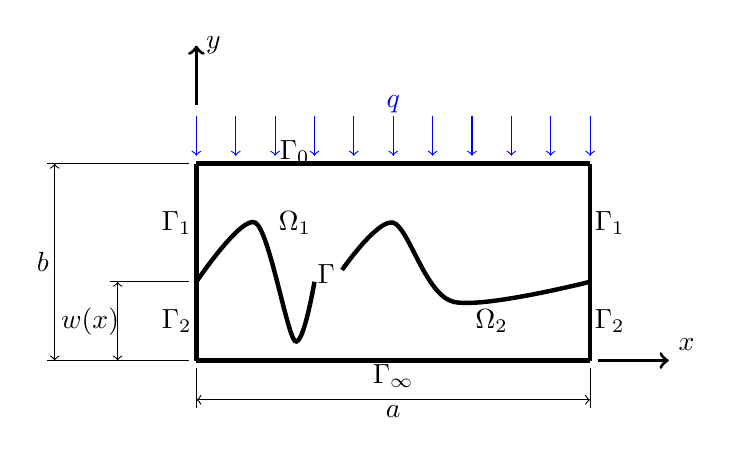
\begin{tikzpicture}[scale=0.5]
		
		\draw [ultra thick] (0, 0) -- (10, 0);
		%\draw [ultra thick] (0, 2) -- (7, 2);
		%\draw [ultra thick] (8, 2) -- (10, 2);
		\draw [ultra thick] plot [smooth] coordinates {(0, 2) (1.5, 3.5) (2.5, 0.5) (3, 2)};
		\draw [ultra thick] plot [smooth] coordinates {(3.7, 2.3) (5, 3.5) (6.5, 1.5) (10, 2)};
		\draw [ultra thick] (0, 5) -- (10, 5);
		\draw [ultra thick] (0, 0) -- (0, 5);
		\draw [ultra thick] (10, 0) -- (10, 5);
		
		\draw (2.5, 3.5) node {$\Omega_1$};
		\draw (7.5, 1) node {$\Omega_2$};	
		\draw (3.3, 2.2) node {$\Gamma$};
		\draw (-0.5, 3.5) node {$\Gamma_1$};
		\draw (-0.5, 1) node {$\Gamma_2$};
		\draw (10.5, 3.5) node {$\Gamma_1$};
		\draw (10.5, 1) node {$\Gamma_2$};
		\draw (5, -0.4) node {$\Gamma_\infty$};
		\draw (2.5, 5.3) node {$\Gamma_0$};
		\draw [blue](5, 6.5) node {$q$};
		\draw (5, -1.3) node {$a$};
		\draw (-3.9, 2.5) node {$b$};
		\draw (-2.7, 1) node {$w(x)$};
		
		\node [above right] at (12, 0) {$x$};
		\node [right] at (0, 8) {$y$};
		
		\draw [->, blue] (0, 6.2) -- (0, 5.2);
		\draw [->, blue] (1, 6.2) -- (1, 5.2);
		\draw [->, blue] (2, 6.2) -- (2, 5.2);
		\draw [->, blue] (3, 6.2) -- (3, 5.2);
		\draw [->, blue] (4, 6.2) -- (4, 5.2);
		\draw [->, blue] (5, 6.2) -- (5, 5.2);
		\draw [->, blue] (6, 6.2) -- (6, 5.2);
		\draw [->, blue] (7, 6.2) -- (7, 5.2);
		\draw [->, blue] (8, 6.2) -- (8, 5.2);
		\draw [->, blue] (9, 6.2) -- (9, 5.2);
		\draw [->, blue] (10, 6.2) -- (10, 5.2);
		
		\draw [->, very thick] (10.2,0) -- (12,0);
		\draw [->, very thick] (0, 6.5) -- (0,8);
		
		\draw [-] (0, -0.2) -- (0, -1.2);
		\draw [-] (10, -0.2) -- (10, -1.2);
		\draw [<->] (0, -1) -- (10, -1);
		
		\draw [-] (-0.2, 0) -- (-3.8, 0);
		\draw [-] (-0.2, 5) -- (-3.8, 5);
		\draw [-] (-0.2, 2) -- (-2.2, 2);
		\draw [<->] (-3.6, 0) -- (-3.6, 5);
		\draw [<->] (-2.0, 0) -- (-2.0, 2);
		
		\end{tikzpicture}
		\caption{Schematic representation of the physical problem}
		\label{fig2}
	\end{center}
\end{figure}
The lateral boundary surfaces $\Gamma_1$ and $\Gamma_2$ from both layers are kept thermally insulated; the bottom surface $\Gamma_\infty$ is subject to a prescribed temperature, and the upper surface $\Gamma_0$ is subject to a prescribed heat flux $q$. The intersection between any plane parallel to the coordinate plane $xy$ and the interface $\Gamma$ generates a curve described by an equation of the form $y = w(x)$. Since the coordinates $x$ and $y$ are directly related along the interface, the TCC will depend only on $x$, that is, $h_c(x, y) \equiv h_c(x)$.

The formulation of the direct steady-state heat conduction problem is given as follows:
\begin{subequations}
	\begin{alignat}{2}
		& \nabla^2 T_1 = 0 \quad\quad\quad\quad && \text{ in } \Omega_1 \label{harm_T1} \\ 
		& -k_1 \frac{\partial T_1}{\partial\mathbf{n}_1} = q && \text{ on } \Gamma_0  \label{cc_T1_2} \\ 
		& \frac{\partial T_1}{\partial \mathbf{n}_1} = 0 && \text{ on }  \Gamma_1 \label{cc_T1_1} \\ 
		& -k_1 \frac{\partial T_1}{\partial\mathbf{n}_1} = h_c(T_1-T_2) \quad\quad\quad\quad && \text{ on }  \Gamma \label{cc_grad_T1} \\ 
		& \nabla^2 T_2 = 0 && \text{ in }  \Omega_2 \label{harm_T2} \\ 
		& \frac{\partial T_2}{\partial \mathbf{n}_2} = 0 && \text{ on }  \Gamma_2 \label{cc_T1_3} \\
		& T_2 = 0 && \text{ on }  \Gamma_\infty \label{cc_T1_4} \\ 
		& k_2\frac{\partial T_2}{\partial\mathbf{n}_2} = - k_1\frac{\partial T_1}{\partial\mathbf{n}_1} && \text{ on }  \Gamma \label{cc_T1_5}
	\end{alignat}
\end{subequations}

In the above equations, $T_1$ and $T_2$ are the temperature fields corresponding to domains $\Omega_1$ and $\Omega_2$ respectively, and the normal unitary vectors $\mathbf{n}_1$ and $\mathbf{n}_2$ point outward the corresponding domains. Particularly at the contact interface $\Gamma$, it can be observed that $\mathbf{n}_1 = -\mathbf{n}_2$.
\\

\noindent{\fontfamily{phv}\selectfont \textbf{INVERSE PROBLEM}}

The inverse problem is the estimation of the function $h_c(x)$ by means of the equation \eqref{definicao_3} on the contact interface $\Gamma$ between the two bodies $\Omega_1$ and $\Omega_2$, according to the physical arrangement illustrated in Fig. \ref{fig2}. The estimation will be performed by using temperature measurements $Y = T(\Gamma_0)$ taken, for example, by an infrared camera on interface $\Gamma_0$. Both surfaces $\Gamma_1$ and $\Gamma_2$ will be kept thermically insulated, and the bottom surface $\Gamma_\infty$ will be subjected to the same prescribed temperature as in the direct problem. The heat flux $q_c(x) = -k_1\frac{\partial T_1}{\partial \mathbf{n}_1}$ and the temperature jump $\Delta T_c(x) = T_1 - T_2$, both evaluated at the contact interface $\Gamma$, will be indirectly estimated by defining and solving two separated auxiliary problems, as proposed by Colaço and Alves\cite{reciproc_3}.
\\

\noindent{\fontfamily{phv}\selectfont \textbf{APPLICATION OF THE RECIPROCITY FUNCTIONAL}}

Based on the idea of reciprocity functional gap developed by Andrieux and Ben Abda\cite{artigo_andrieux}, Colaço and Alves\cite{reciproc_3} introduced the concept of Reciprocity Functional (RF) through the following expression:
\begin{align}
	\Re(F) = \int_{\Gamma_0}\left[\left(\frac{-q}{k_1}\right)F - Y\frac{\partial F}{\partial\mathbf{n_1}}\right]d\Gamma_0
	\label{def_funcional_reciprocidade}
\end{align}
where $F$ is a harmonic function defined over $\Omega_1$, and $Y$ represents the measured temperatures along the upper boundary surface $\Gamma_0$.

Colaço and Alves\cite{reciproc_3} formulated two diffusive problems for determining two classes of auxiliary functions $F_1$ and $G_1$, over the same domain $\Omega_1$. Combining the direct problem expressed in \eqref{harm_T1}--\eqref{cc_T1_5} with the auxiliary problems and their boundary conditions, and applying Green's second theorem, they were able to demonstrate the following identities, which relate the temperature jump and the heat flux at the inaccessible interface $\Gamma$ to the measured temperatures $Y$ along the external surface $\Gamma_0$:
\begin{align}
	k_1\int_{\Gamma_0}\left[\left(\frac{-q}{k_1}\right)\right. & \left.F_1 - Y\frac{\partial F_1}{\partial\mathbf{n_1}}\right]d\Gamma_0
	= \nonumber \\
	& \int_\Gamma k_1 \frac{\partial F_1}{\partial\mathbf{n_1}}\left(T_1 - T_2\right)d\Gamma
	\label{identidade_T} \\ \nonumber \\
	k_1\int_{\Gamma_0}\left[\left(\frac{-q}{k_1}\right)\right. & \left.G_1 -  Y\frac{\partial G_1}{\partial\mathbf{n_1}}\right]d\Gamma_0
	= \nonumber \\
	& \int_\Gamma -k_1 G_1 \frac{\partial T_1}{\partial\mathbf{n_1}}d\Gamma
	\label{identidade_q}
\end{align}

Now let $k_1 \frac{\partial F}{\partial\mathbf{n_1}}$, $T_1 - T_2$, $G$ and $-k_1 \frac{\partial T_1}{\partial\mathbf{n_1}}$ belong to a linear space of functions $L^2(\Gamma)$, and let the inner product in this linear space be defined as:
\begin{align}
	\langle f_1, f_2\rangle_{L^2(\Gamma)} = \int_\Gamma f_1(\Gamma) f_2(\Gamma) d\Gamma \label{definicao_innner_product}
\end{align} 

By rasing two families of auxiliary functions $F_{1,j}, j=1,2,\ldots N_1$ and $G_{1,j}, j=1,2,\ldots N_2$ from the corresponding auxiliary problems, and using the definition of inner product in \eqref{definicao_innner_product}, as well as the definition of the RF in \eqref{def_funcional_reciprocidade}, expressions \eqref{identidade_T} and \eqref{identidade_q} may be rewritten as:
\begin{align}
	& k_1 \Re(F_{1,j})
	=
	\left\langle \left[T_1 - T_2\right]_\Gamma, \beta_j\right\rangle _{L^2(\Gamma)}
	\label{identidade_T_inner} \\
	& k_1 \Re(G_{1,j})
	=
	\left\langle  -k_1 \frac{\partial T_1}{\partial\mathbf{n_1}}\bigg|_\Gamma, \gamma_j\right\rangle _{L^2(\Gamma)}
	\label{identidade_q_inner}
\end{align}
where
\begin{align}
	& \beta_j = k_1 \frac{\partial F_{1,j}}{\partial\mathbf{n_1}}\bigg|_\Gamma \label{expressao_define_beta} \\
	& \gamma_j = G_{1,j}\big|_\Gamma \label{expressao_define_gamma}
\end{align}

Assuming that $\beta_j, j=1,2,\ldots N_1$ and $\gamma_j, j=1,2,\ldots N_2$ form two sets of orthonormal functions, they define two linear subspaces over which $T_1 - T_2$ and $-k_1 \frac{\partial T_1}{\partial\mathbf{n_1}}$ may be ortogonally projected, that is:
\begin{align}
	& [T_1 - T_2]_\Gamma \approx \sum_{j=1}^{N_1} \left\langle  \left[T_1 - T_2\right]_\Gamma, \beta_j \right\rangle_{L^2(\Gamma)} \beta_j \\ 
	& - k_1 \frac{\partial T_1}{\partial\mathbf{n_1}}\bigg|_\Gamma \approx \sum_{j=1}^{N_2} \left\langle  -k_1 \frac{\partial T_1}{\partial\mathbf{n_1}}\bigg|_\Gamma, \gamma_j \right\rangle_{L^2(\Gamma)} \gamma_j
\end{align}

Applying identities \eqref{identidade_T_inner} and \eqref{identidade_q_inner} to the above equations, and assuming that the orthogonal projections represent the corresponding functions in a reasonable manner, the following relations can be written:
\begin{align}
	& [T_1 - T_2]_\Gamma = \sum_{j=1}^{N_1} k_1 \Re(F_{1,j}) \beta_j \label{resultado_1} \\
	& - k_1 \frac{\partial T_1}{\partial\mathbf{n_1}}\bigg|_\Gamma = \sum_{j=1}^{N_2} k_1 \Re(G_{1,j}) \gamma_j \label{resultado_2}
\end{align}

The substitution of these results into the definition of the TCC \eqref{definicao_3} leads to:
\begin{align}
	& h_c(x) % = \frac{- k_1 \displaystyle\frac{\partial T_1}{\partial\mathbf{n_1}}\bigg|_\Gamma}{[T_1 - T_2]_\Gamma} 
	= \frac{\displaystyle\sum_{j=1}^{N_2} \Re(G_{1,j}) \gamma_j(x)}{\displaystyle\sum_{j=1}^{N_1} \Re(F_{1,j}) \beta_j(x)}
	\label{equacao_definicao_f_r}
\end{align}

The expression \eqref{equacao_definicao_f_r} allows the estimation of the TCC distribution along the contact interface $\Gamma$, by knowing the distribution of temperatures $Y$ measured along the external interface $\Gamma_0$, thus eliminating the previous need of knowing internal characteristics of the composite body, confirming the non-intrusive feature of the method. The families of functions $F_{1, j}$ and $G_{1, j}$, and the integrals that provide the Reciprocity Functional values envolving these functions, need to be calculated just once for a certain geometric and thermophysical characterization of the problem, so that the method is also non-iterative.
\\

\noindent{\fontfamily{phv}\selectfont \textbf{FORMULATION AND SOLUTION OF THE AUXILIARY PROBLEM}}
\\

\noindent{\fontfamily{phv}\selectfont \textbf{First auxiliary problem: estimation of the temperature jump at the contact interface}}

Let $F_{1,j}$ and $F_{2,j}$ be two families of harmonic functions, defined over the domains $\Omega_1$ and $\Omega_2$ respectively, and let $\psi_j(x), j=1,2,\ldots N_1$ be a family of linear independent functions. The first auxiliary problem, as proposed by Abreu \textit{et al.}\cite{artigo_abreu_3}, may be defined as follows:
\begin{subequations}
	\begin{alignat}{2}
		& \nabla^2 F_{1,j} = 0 \quad\quad\quad\quad\quad && \text{ in } \Omega_1 \label{funcao_F_harm_T1} \\
		& F_{1,j} = \psi_j && \text{ on } \Gamma_0  \label{funcao_F_cc_T1_2} \\
		& \frac{\partial F_{1,j}}{\partial \mathbf{n}_1} = 0 && \text{ on }  \Gamma_1 \label{funcao_F_cc_T1_1} \\ 
		& F_{1,j} = F_{2, j} \quad\quad\quad\quad\quad\quad\quad\quad && \text{ on }  \Gamma \label{funcao_F_cc_grad_T1} \\
		& \nabla^2 F_{2,j} = 0 && \text{ in }  \Omega_2 \label{funcao_F_harm_T2} \\
		& \frac{\partial F_{2,j}}{\partial \mathbf{n}_2} = 0 && \text{ on }  \Gamma_2 \label{funcao_F_cc_T1_3} \\
		& F_{2,j} = 0 && \text{ on }  \Gamma_\infty \label{funcao_F_cc_T1_4} \\
		& k_2\frac{\partial F_{2, j}}{\partial\mathbf{n}_2} = - k_1\frac{\partial F_{1,j}}{\partial\mathbf{n}_1} && \text{ on }  \Gamma \label{funcao_F_cc_T1_5}
	\end{alignat}
\end{subequations}
\\

\noindent{\fontfamily{phv}\selectfont \textbf{Second auxiliary problem: estimation of the heat flux at the contact interface}}

Let $G_{1,j}$ be a family of harmonic functions, defined over the domain $\Omega_1$, and let $\phi_j(x), j=1,2,\ldots N_2$ be a family of linear independent functions. The second auxiliary problem, as proposed by Abreu \textit{et al.}\cite{artigo_abreu_3}, may be defined as follows:
\begin{subequations}
	\begin{alignat}{2}
		& \nabla^2 G_{1,j} = 0 \quad\quad\quad\quad\quad && \text{ in } \Omega_1 \label{funcao_G_harm_T1} \\ 
		& G_{1,j} = \phi_j && \text{ on } \Gamma_0  \label{funcao_G_cc_T1_2} \\
		& \frac{\partial G_{1,j}}{\partial \mathbf{n}_1} = 0 && \text{ on }  \Gamma_1 \label{funcao_G_cc_T1_1} \\ 
		& \frac{\partial G_{1,j}}{\partial\mathbf{n}_1} = 0 \quad\quad\quad\quad\quad\quad\quad\quad && \text{ on }  \Gamma \label{funcao_G_cc_grad_T1}
	\end{alignat}
\end{subequations}
\\

\noindent{\fontfamily{phv}\selectfont \textbf{Solution of the auxiliary problems using CITT}}

The Classic Integral Transform Technique (CITT) provides a systematic and efficient approach for solving linear diffusive problems envolving nonhomogeneous terms in the differential equations or in the boundary conditions\cite{livro_integral_transforms_cotta}, and was employed by Padilha \textit{et al.}\cite{artigo_padilha_3} for the solution of the auxiliary problems formulated in the previous subsections, specifically for the case of the planar horizontal contact interface. Since the current study comprises a more general configuration, still keeping the basic thermophysical and geometrical characteristics, that method was a natural choice for solving its corresponding auxiliary problems.

In order to solve equations \eqref{funcao_F_harm_T1} to \eqref{funcao_F_cc_T1_5} and \eqref{funcao_G_harm_T1} to \eqref{funcao_G_cc_grad_T1} by the CITT method, it is necessary to define the following integral transforms and inversion formulas\cite{livro_integral_transforms_cotta} in the $x$-direction, where the boundary conditions are homogeneous:
\begin{itemize}
	\item Functions $F_{1, j}$ and $F_{2, j}$:
	\begin{subequations}
		\begin{align}
		& \bar{F}_{1,j,m}(y) = \int_0^a F_{1, j}(x, y) X(\mu_m, x) dx \label{definicao_da_transf_F1}  \\
		& F_{1, j}(x, y) = \sum_{m=0}^\infty \frac{X(\mu_m, x)}{N(\mu_m)}\bar{F}_{1,j,m}(y) \label{definicao_da_transf_inv_F1}	 \\
		& \bar{F}_{2,j,m}(y) = \int_0^a F_{2, j}(x, y) X(\mu_m, x) dx \label{definicao_da_transf_F2}  \\
		& F_{2, j}(x, y) = \sum_{m=0}^\infty \frac{X(\mu_m, x)}{N(\mu_m)}\bar{F}_{2,j,m}(y) \label{definicao_da_transf_inv_F2}	
		\end{align}
	\end{subequations}
	\item Functions $G_{1, j}$:
	\begin{subequations}
		\begin{align}
		& \bar{G}_{1,j,m}(y) = \int_0^a G_{1, j}(x, y) X(\mu_m, x) dx \label{definicao_da_transf_G1}  \\
		& G_{1, j}(x, y) = \sum_{m=0}^\infty \frac{X(\mu_m, x)}{N(\mu_m)}\bar{G}_{1,j,m}(y) \label{definicao_da_transf_inv_G1}		
		\end{align}
	\end{subequations}
\end{itemize}

In the above equations, $X(\mu_m, x)$ are the eigenfunctions of the following associate eigenvalue problem\cite{livro_integral_transforms_cotta}:
\begin{subequations}
	\begin{alignat}{2}
	& \frac{d^2 X(\mu_m, x)}{d x^2} + \mu_m^2 X(\mu_m, x) = 0, && 0 < x < a \label{problema_vc_1a} \\
	& \frac{d X(\mu_m, x)}{d x} = 0 && x = 0 \label{problema_vc_1b} \\
	& \frac{d X(\mu_m, x)}{d x} = 0 && x = a \label{problema_vc_1c}
	\end{alignat}
\end{subequations}
and the norm $N(\mu_m)$ is given as\cite{livro_integral_transforms_cotta}:
\begin{align}
N(\mu_m) = \left\lbrace
\begin{array}{ll}
a, \quad\quad\quad\quad & m = 0 \\ \\
\frac{a}{2}, & m = 1,2,3,\ldots
\end{array}
\right. \label{valor_integral_norm}
\end{align}

The solution of \eqref{problema_vc_1a} is given as\cite{livro_integral_transforms_cotta}:
\begin{align}
& X(\mu_m, x) = \left\lbrace
\begin{array}{ll}
1, & m = 0 \\ \\
\cos \mu_m x, & m = 1,2,3,\ldots
\end{array}
\right . \label{definicao_das_autofuncoes}
\end{align}
where the eigenvalues $\mu_m$ are given as\cite{livro_integral_transforms_cotta}:
\begin{align}
\mu_m = \left\lbrace
\begin{array}{ll}
0, \quad\quad\quad\quad & m = 0 \\ \\
\frac{m\pi}{a}, & m = 1,2,3,\ldots
\end{array}
\right.
\end{align}

Applying the integral transform to the partial differential equations \eqref{funcao_F_harm_T1}, \eqref{funcao_F_harm_T2} and \eqref{funcao_G_harm_T1}, the dependency on $x$ is eliminated, and the following ordinary equations in $y$ are obtained:
\begin{align}
& \frac{d^2 \bar{F}_{1,j,m}(y)}{d y^2}
-
\mu_m^2 \bar{F}_{1,j,m}(y) = 0 \label{eq_dif_ord_F1} \\
& \frac{d^2 \bar{F}_{2,j,m}(y)}{d y^2}
-
\mu_m^2 \bar{F}_{2,j,m}(y) = 0 \label{eq_dif_ord_F2} \\
& \frac{d^2 \bar{G}_{1,j,m}(y)}{d y^2}
-
\mu_m^2 \bar{G}_{1,j,m}(y) = 0 \label{eq_dif_ord_G1}
\end{align}

Applying the integral transform to the boundary conditions \eqref{funcao_F_cc_T1_2}, \eqref{funcao_F_cc_T1_4} and \eqref{funcao_G_cc_T1_2}, and using the resulting conditions for solving the above differential equations, the following general solutions may be found\cite{livro_boyce}:
\begin{align}
& \bar{F}_{1,j,m}(y) = \mathbb{A}_{j,m} \frac{\sinh\mu_m (b - y)}{\sinh\mu_m b} +	\bar{\psi}_{j, m}\frac{\sinh\mu_m y}{\sinh\mu_m b} \label{solucao_temporaria_F1} \\
& \bar{F}_{2,j,m}(y) = \mathbb{D}_{j,m}\frac{\sinh\mu_m y}{\sinh\mu_m b} \label{solucao_temporaria_F2} \\
& \bar{G}_{1,j,m}(y) = \mathbb{E}_{j,m} \frac{\sinh\mu_m (b - y)}{\sinh\mu_m b} +\bar{\phi}_{j, m}\frac{\sinh\mu_m y}{\sinh\mu_m b} \label{solucao_temporaria_G1}
\end{align}
where $\bar{\psi}_{j, m}$ and $\bar{\phi}_{j, m}$ are the integral transforms of $\psi_j(x)$ and $\phi_j(x)$, and $\mathbb{A}_{j,m}$, $\mathbb{D}_{j,m}$ and $\mathbb{E}_{j,m}$ are constants to be determined.

In order to evaluate those constants, the inverse formulas \eqref{definicao_da_transf_inv_F1}, \eqref{definicao_da_transf_inv_F2} and \eqref{definicao_da_transf_inv_G1} must be substituted into boundary conditions \eqref{funcao_F_cc_grad_T1}, \eqref{funcao_F_cc_T1_5} and \eqref{funcao_G_cc_grad_T1}, and the resulting expressions must be transformed, which leads to an infinite linear system for $\mathbb{A}_{j,m}$ and $\mathbb{D}_{j,m}$ as follows:
\begin{subequations}
\begin{align}
& \sum_{m = 0}^\infty \bar{a}_{n,m} \mathbb{A}_{j,m} + \sum_{m = 0}^\infty \bar{b}_{n,m} \mathbb{D}_{j,m} = \bar{c}_{n,j} \label{sistema_para_coeficientes_1}
\end{align}
\begin{align}
& \sum_{m = 0}^\infty \bar{p}_{n,m} \mathbb{A}_{j,m} + \sum_{m = 0}^\infty \bar{q}_{n,m} \mathbb{D}_{j,m} = \bar{r}_{n,,j} \label{sistema_para_coeficientes_2}
\end{align}
\end{subequations}
and an inifinite linear system for $\mathbb{E}_{j,m}$ as follows:
\begin{align}
& \sum_{m = 0}^\infty \bar{u}_{n,m} \mathbb{E}_{j,m} = \bar{v}_{n,j} \label{sistema_para_coeficientes_3}
\end{align}
where $\bar{a}_{n,m}$, $\bar{b}_{n,m}$, $\bar{c}_{n,j}$, $\bar{p}_{n,m}$, $\bar{q}_{n,m}$, $\bar{r}_{n,j}$, $\bar{u}_{n,m}$ and $\bar{v}_{n,j}$ are constants calculated by the integral transforms of expressions that depend on $w(x)$.

By truncating the infinite sums up to a limiting index $M$, the linear systems \eqref{sistema_para_coeficientes_1}-\eqref{sistema_para_coeficientes_2} and \eqref{sistema_para_coeficientes_3} may be numerically solved to obtain the unknown constants $\mathbb{A}_{j,m}$, $\mathbb{D}_{j,m}$ and $\mathbb{E}_{j,m}$.

The functions $\beta_j(x)$ and $\gamma_j(x)$, required for the estimation of the TCC through equation \eqref{equacao_definicao_f_r}, may be calculated by substituting the previous results in definitions \eqref{expressao_define_beta} and \eqref{expressao_define_gamma}, which gives:
\begin{align}
& \beta_j(x) = \frac{k_1}{\sqrt{1 + w'(x)^2}}\left\lbrace \frac{\mathbb{A}_{j,0} - \bar{\psi}_{j,0}}{ab} +
\frac{2}{a}\sum_{m=1}^M \mu_m \right. \nonumber \\
& \left[ \mathbb{A}_{j,m}\frac{\scriptstyle\cos\mu_m x\cosh\mu_m v(x) - w'(x)\sin\mu_m x\sinh\mu_m v(x)}{\scriptstyle\sinh\mu_m b} \right. - \nonumber \\
&\left. \left. \bar{\psi}_{j, m}\frac{\scriptstyle w'(x)\sin\mu_m x\sinh\mu_m w(x) + \cos\mu_m x\cosh\mu_m w(x)}{\scriptstyle\sinh\mu_m b}\right] \right\rbrace
\label{serie_para_beta}
\end{align}
\begin{align}
\gamma_j(x) = & \frac{\mathbb{E}_{j,0}[b - w(x)] + \bar{\phi}_{j,0}w(x)}{ab} + \nonumber \\
& \frac{2}{a}\sum_{m=1}^M \left\lbrace\mathbb{E}_{j,m}\frac{\sinh\mu_m [b - w(x)]}{\sinh\mu_m b} + \right. \nonumber \\
& \left. \bar{\phi}_{j, m}\frac{\sinh\mu_m w(x)}{\sinh\mu_m b}\right\rbrace \cos\mu_m x
\label{serie_para_gamma}
\end{align} 
where $v(x) = b - w(x)$.
\\

\noindent{\fontfamily{phv}\selectfont \textbf{Orthonormalization of the auxiliary functions}}

The orthonormality of functions $\beta_j(x)$ and $\gamma_j(x)$ was a prerequisite for applying the expansions \eqref{resultado_1} and \eqref{resultado_2}, which provide the necessary estimatives for the temperature jump and heat flux at the contact interface. At first, this feature cannot be guaranteed for the functions $\beta_j(x)$ and $\gamma_j(x)$ obtained from the previous subsection. However, assuming that the sets of functions $\beta_j(x), j=1,2,\dots, N_1$ and $\gamma_j(x), j=1,2,\dots, N_2$ are linearly independent, it is possible to obtain a new set of functions $\hat{\beta}_j(x)$ and $\hat{\gamma}_j(x)$ fulfilling that condition, by means of the Gram-Schmidt orthonormalization algorithm:
\begin{align}
\hat{\beta}_j = & \frac{1}{\norm{\nu_j}}\beta_j - \sum_{k=0}^{j-1} \frac{\langle \beta_j, \hat{\beta}_k \rangle_{L^2(\Gamma)}}{\norm{\nu_j}} \hat{\beta}_k \label{termo_beta} , \\
& j=1,2,\dots, N_1 
\end{align}
\begin{align}
\hat{\gamma}_j = & \frac{1}{\norm{\upsilon_j}}\gamma_j - \sum_{k=0}^{j-1} \frac{\langle \gamma_j, \hat{\gamma}_k \rangle_{L^2(\Gamma)}}{\norm{\upsilon_j}} \hat{\gamma}_k \label{termo_gamma},  \\
& j=1,2,\dots, N_2 \nonumber 
\end{align}
where
\begin{align}
& \nu_j = \beta_j - \sum_{k = 0}^{j - 1} \langle \beta_j, \hat{\beta}_k\rangle_{L^2(\Gamma)}\hat{\beta}_k \\
& \upsilon_j = \gamma_j - \sum_{k = 0}^{j - 1} \langle \gamma_j, \hat{\gamma}_k\rangle_{L^2(\Gamma)}\hat{\gamma}_k
\end{align}

Due to the linearity of the auxiliary problems, the corresponding constants $\hat{\mathbb{A}}_{j,m}$ and $\hat{\mathbb{E}}_{j,m}$ may be obtained from an analogous procedure:
\begin{align}
\hat{\mathbb{A}}_{j,m} = & \frac{1}{\norm{\nu_j}} \mathbb{A}_{j,m} - \sum_{k=0}^{j-1} \frac{\langle \beta_j, \hat{\beta}_k \rangle}{\norm{\nu_j}} \hat{\mathbb{A}}_{k,m}
\label{expressao_relaciona_psi} ,\\
& j=1,2,\dots, N_1; m=0,1,2,\ldots,M
\end{align}
\begin{align}
\hat{\mathbb{E}}_{j,m} = & \frac{1}{\norm{\upsilon_j}} \mathbb{E}_{j,m} - \sum_{k=0}^{j-1} \frac{\langle \gamma_j, \hat{\gamma}_k \rangle}{\norm{\upsilon_j}} \hat{\mathbb{E}}_{k,m}
\label{expressao_relaciona_zeta} , \\
& j=1,2,\dots, N_2 ; m=0,1,2,\ldots,M  \nonumber 
\end{align}

Equations \eqref{expressao_relaciona_psi} and \eqref{expressao_relaciona_zeta} are basically recurrence relations that allow determination of coefficients $\hat{\mathbb{A}}_{j,m}$ and $\hat{\mathbb{E}}_{j,m}$ from coefficients $\mathbb{A}_{j,m}$ and $\mathbb{E}_{j,m}$, which have to be previously calculated as the solution of the linear systems \eqref{sistema_para_coeficientes_1}-\eqref{sistema_para_coeficientes_2} and \eqref{sistema_para_coeficientes_3}. These new coefficients, when substituted into \eqref{serie_para_beta} and \eqref{serie_para_gamma} at each step of the recurrency process, will provide the functions $\hat{\beta}_j$ and $\hat{\gamma}_j$ that meet the orthonormality criteria. From this point on, for the sake of simplicity, the symbol $\hat{}$ will be dropped, and the coefficients $\mathbb{A}_{j,m}$ and $\mathbb{E}_{j,m}$ will be considered as been calculated after the orthonormality procedure, as well as the functions $F_{1,j}$, $G_{1,j}$, $\beta_j$ and $\gamma_j$.
\\

\noindent{\fontfamily{phv}\selectfont \textbf{ANALYTICAL FORMULATION FOR THE THERMAL CONDUCTANCE}}

Once the family of functions $F_{1,j}$ and $G_{1,j}$ have been determined, they can be replaced into the definition \eqref{def_funcional_reciprocidade}, in order to obtain the following expressions for their respective Reciprocity Functionals:
\begin{align}
\Re(F_{1,j})
& =
-\frac{q}{k_1}\bar{\psi}_{j,0} + \frac{\mathbb{A}_{j,0} - \bar{\psi}_{j,0}}{b} \bar{y}_0 + \nonumber \\
&\sum_{m=1}^M \mu_m \left(\frac{\mathbb{A}_{j,m}}{\sinh\mu_m b} - \frac{\bar{\psi}_{j, m}}{\tanh\mu_m b}\right)\bar{y}_m
\label{calculo_FR_F1_antes_b} 
\end{align}
\begin{align}
\Re(G_{1,j})
& =
-\frac{q}{k_1}\bar{\phi}_{j,0} + \frac{\mathbb{E}_{j,0} - \bar{\phi}_{j,0}}{b} \bar{y}_0 + \nonumber \\
& \sum_{m=1}^M \mu_m \left(\frac{\mathbb{E}_{j,m}}{\sinh\mu_m b} - \frac{\bar{\phi}_{j, m}}{\tanh\mu_m b}\right)\bar{y}_m
\label{calculo_FR_G1_antes_b}
\end{align}
where $\bar{y}_0$ and $\bar{y}_m$ are given as:
\begin{align}
& \bar{y}_0 = \frac{1}{a}\int_0^a Y(x) dx \label{coef_it_0} \\ 
& \bar{y}_m = \frac{2}{a}\int_0^a Y(x) \cos\mu_m x dx, m = 1, 2, ..., M \label{coef_it_m}
\end{align}

Equations \eqref{calculo_FR_F1_antes_b} and \eqref{calculo_FR_G1_antes_b} provide the RFs given by $\Re(F_{1,j})$ and $\Re(G_{1,j})$ for a particular choice of functions $\psi_j(x)$ and $\phi_j(x)$. In the present work, these functions were the same as the ones chosen for the study conducted by Padilha \textit{et al.}\cite{artigo_padilha_3} for the case of the horizontal planar contact interface:
\begin{align}
\psi_j(x), \phi_j(x) = \left\lbrace
\begin{array}{ll}
\sqrt{\frac{1}{a}}, & j = 0 \\ 
\sqrt{\frac{2}{a}}\cos \mu_j x, & j = 1,2,3,\ldots
\end{array}
\right.
\end{align} 

Finally, having the values of the RFs, as well as the orthonormal base functions $\beta_j(x)$ and $\gamma_j(x)$, the estimative of the TCC can be calculated at any point $x$ in $0 \le x \le a$ by substituting into equation \eqref{equacao_definicao_f_r}, repeated below:
\begin{align}
& h_c(x) % = \frac{- k_1 \displaystyle\frac{\partial T_1}{\partial\mathbf{n_1}}\bigg|_\Gamma}{[T_1 - T_2]_\Gamma} 
= \frac{\displaystyle\sum_{j=1}^{N_2} \Re(G_{1,j}) \gamma_j(x)}{\displaystyle\sum_{j=1}^{N_1} \Re(F_{1,j}) \beta_j(x)}
\label{equacao_definicao_f_r_rep}
\end{align}

Equations \eqref{calculo_FR_F1_antes_b} and \eqref{calculo_FR_G1_antes_b}, as well as equation \eqref{equacao_definicao_f_r_rep}, represent a generalization of the algebraic expression obtained by Padilha \textit{et al.}\cite{artigo_padilha_3} for the particular case of the horizontal planar interface contact corresponding to the assembly in Fig. \ref{fig2}. It is important to highlight that the RFs given by $\Re(F_{1,j})$ and $\Re(G_{1,j})$ depend on the coefficients $\mathbb{A}_{j,m}$ and $\mathbb{E}_{j,m}$, which need to be calculated only once for a particular thermophysical and geometric configuration.

From a practical point of view, once the measured temperatures $Y$ along the boundary surface $\Gamma_0$ are evaluated at discrete points, the analytical form of the function $Y(x)$ is not known. However, as suggested by Mocerino \textit{et al.}\cite{artigo_mocerino}, it can be approximated by a Fourier series expansion of the form:
\begin{align}
Y(x) \approx \bar{y}_0 + \sum_{m=1}^M \bar{y}_m \cos\mu_m x \label{aproximacao_Y}
\end{align}
where the coefficients $\bar{y}_0$ and $\bar{y}_m$ are exactly those expressed in \eqref{coef_it_0} and \eqref{coef_it_m}. Thus, a least-square procedure may be employed in order to numerically calculate $\bar{y}_0$ and $\bar{y}_m$ from a set of samples $(x_i, Y_i)$, each one corresponding to a position along the upper boundary $\Gamma_0$ and the measured temperature at that point.
\\

\noindent{\fontfamily{phv}\selectfont \textbf{COMPUTATIONAL IMPLEMENTATION AND NUMERICAL RESULTS}}

In this work, in order to verify the analytical results of the previous sections, the experimental apparatus of Fig. \ref{fig2} has been simulated, both for the direct problem and for the inverse problem. Table \ref{tabela_params} summarizes the numerical values of the relevant parameters which were adopted. 

The following procedure has been followed:
\begin{enumerate}
	\item Different theoretical geometries of contact interface were proposed; for each geometry, a corresponding expression of the form $y = w(x)$ was defined. The geometries are summarized in Table \ref{tabela_interfaces};
	\item Different theoretical distribution profiles for the TCC were proposed; for each profile, a corresponding expression for $h_c(x)$ was defined. The profiles are summarized in Table \ref{tabela_ctc};
	\item The direct problem defined in equations \eqref{harm_T1} to \eqref{cc_T1_5} was numerically solved for each combination of a geometry and a TCC profile, leading to a collection of possible temperature distributions over the domain as a result;
	\item From each temperature distribution, samples were taken along the upper boundary interface $\Gamma_0$ of the experimental assembly, providing the set of temperature values $Y$ required by the inverse problem. Gaussian noises were introduced in the simulated temperatures, simulating measurement errors;
	\item Equation \eqref{equacao_definicao_f_r_rep} was used to estimate the TCC along the interface contact and compared to the expected profile. This comparison was made for each combination of interface contact geometry and theoretical TCC profile. The equation for the interface contact $w(x)$ was used to calculate the coefficients $\mathbb{A}_{j,m}$ and $\mathbb{E}_{j,m}$ from the linear systems \eqref{sistema_para_coeficientes_1}, \eqref{sistema_para_coeficientes_2} and \eqref{sistema_para_coeficientes_3}. The synthetic temperature measuremens $Y$ were used in expression \eqref{aproximacao_Y}, which yields the values for $\bar{y}_0$ and $\bar{y}_m$ to be used in the RF expressions \eqref{calculo_FR_F1_antes_b} and \eqref{calculo_FR_G1_antes_b}.
\end{enumerate}

\begin{table}[H]
	\centering
	\caption{Parameters used in the test problems}
	\begin{tabular}{|l|l|}
		\hline
		\textbf{Parameter} & \textbf{Value}  \\ \hline
		$a$       & 0.04 m   \\ \hline
		$b$       & 0.02 m     \\ \hline
		$k_1$     & 54 W/(m \celsius)  \\ \hline
		$k_2$     & 14 W/(m \celsius) \\ \hline
		$q$       & -100,000 W/$\text{m}^2$ \\ \hline
		$h_{max}$       & 1000 W/($\text{m}^2$ \celsius) \\ \hline
	\end{tabular}		
	\label{tabela_params}
\end{table}

\begin{table}[H]
	\centering
	\caption{Contact interface geometries}
	\begin{tabular}{|l|l|}
		\hline 
		\textbf{Geometry} & \textbf{Expression for} $w(x)$    \\ \hline
		1       & $\frac{b}{2}$   \\ \hline
		2       & $\begin{array}{ll}
		\frac{19bx^2}{8a^2}-\frac{7bx}{24a}+\frac{b}{2}, &  0 \le x < \frac{a}{3} \\
		 -\frac{25bx^2}{8a^2}+\frac{27bx}{8a}-\frac{b}{9}, &  \frac{a}{3} \le x < \frac{2a}{3} \\ 
		 \frac{bx^2}{8a^2}-\frac{23bx}{24a}+\frac{4b}{3}, &  \frac{2a}{3} \le x \le a
		\end{array}$     \\ \hline
		3       & $ \frac{b}{2} + \frac{1}{20} \cos\frac{4 \pi  x}{a}$ \\ \hline
	\end{tabular}			
	\label{tabela_interfaces}
\end{table}

\begin{table}[H]
	\centering
	\caption{Theoretical thermal contact conductance profiles}
	\begin{tabular}{|l|l|}
		\hline
		\textbf{Profile} & $h_c(x)$[W/($\text{m}^2$ \celsius)]  \\ \hline
		\multirow{2}{*}{1} & $h_{max}$, $x < a/4$ e $x > 3a/4$ \\ & 0, $a/4 < x < 3a/4$ \\ \hline
		2 & $h_{max}\sin\frac{\pi x}{a}$ \\ \hline
		\multirow{3}{*}{3} & $h_{max}/2$, $x < a/4$ and $a/2 < x < 3a/4$ \\ & $h_{max}$, $a/4 < x < a/2$ \\ & 0, $ x > 3a/4$
		\\ \hline
	\end{tabular}			
	\label{tabela_ctc}
\end{table}

The experimental noises in step 4 were generated according to the following equation:
\begin{align}
\tilde{\mathbf{Y}} = \mathbf{Y} + \mathbf{\varepsilon} \sigma \label{modelagem_erro}
\end{align}
where $\mathbf{Y}$ is the set of exact temperatures, $\tilde{\mathbf{Y}}$ is the set of temperatures with erros, $\sigma$ is the standard deviation of the temperature measures, and $\epsilon$ is a Gaussian random variable with zero mean and unity variance. Three different values of $\sigma$ were tried: $\sigma = \text{0.0}\celsius$ (corresponding to synthetic temperatures with no measuremente errors), $\sigma = \text{0.1}\celsius$ and $\sigma = \text{0.5}\celsius$.

Due to lack of space, not all results from all interface geometries tested will be discussed in this work. Instead, the specific case of the geometry 2 was chosen to be discussed here. The format of the contact interface may be observed in Fig. \ref{fig3}. The results found for this case are shown in Figs. \ref{figura_ctc_interface_02a} to \ref{figura_ctc_interface_02c}.
\begin{figure}[H]
	\begin{center}
		\begin{tikzpicture}
		\begin{axis}[
		anchor=east,  
		ticks=none,
		width=8cm,
		height=4cm,
		%ylabel=Iterações Lineares,
		xmin = 0,
		xmax = 0.04,
		ymin = 0,
		ymax = 0.02]
		\pgfplotstableread{../data/interface_02.dat} 
		\teff
		\addplot[color=blue,mark=none,smooth] table from \teff;
		\end{axis}
		\end{tikzpicture}
		\caption{Geometry for contact interface 3}
		\label{fig3}
	\end{center}
\end{figure}
It is possible to notice that the estimated profiles for the TCC show a very good adherence to the theoretical ones. For the simulations using $\sigma = \text{0.0}\celsius$, corresponding to temperature measurements without noise, there is an excellent agreement between the estimated and expected profiles. For the other cases, in which gaussian noises were added, the general behavior of the TCC was well captured. A direct relationship between the amplitude of the noise and the exactness of the estimative was also observed: as the amplitude of the noise diminishes, the estimatives become closer to the exact values.

An improvement of the calculated estimatives was also observed, as more terms were added to the expressions on the numerator and denominator of the equation \eqref{equacao_definicao_f_r_rep}, until a certain limit of the number of terms was achieved. From that point on, as more terms were included in the summations, the estimatives diverged quickly, leading to unstable results. However, when comparing to the results found by Padilha \textit{et al.}\cite{artigo_padilha_3}, the maximum number of terms in the summations ($N_1=N_2=20$) were greater than those used in that work ($N_1=N_2=14$), in which the same stability problems were present, and the sampled temperatures $Y$ were represented by a \textit{spline} instead of a Fourier expansion. Since both temperature jumps and heat flux at the contact interface were represented by summations with more terms, the estimates were more accurate as well.

Due to the non-intrusive nature of the method, as well as the use of several optimizations (specially in the Gram-Schmidt orthonormalization), the computational implementation showed a very fast processing time. In the simulations executed in this work, using an Intel Core\textsuperscript{\texttrademark} i5-8250U CPU 1.60 GHz, processing times for each profile estimation ranged from 2.0 seconds to 2.4 seconds.
\begin{figure}[H]
	\graficoctc{02}{01}{1}{a}
	\caption{Estimated TCC for contact interface geometry 2 and TCC profile 1 using synthetic data and the reciprocity functional approach for $\sigma = \text{0.0}\celsius$ ($\textcolor{blue}{\ocircle}$), $\sigma = \text{0.1}\celsius$ ($\textcolor{red}{\square}$) and $\sigma = \text{0.5}\celsius$ ($\textcolor{gray}{\triangle}$), and the exact profiles ($\text{--}$)}
	\label{figura_ctc_interface_02a}
\end{figure}
\begin{figure}[H]
	\graficoctc{02}{02}{2}{b}
	\caption{Estimated TCC for contact interface geometry 2 and TCC profile 2 using synthetic data and the reciprocity functional approach for $\sigma = \text{0.0}\celsius$ ($\textcolor{blue}{\ocircle}$), $\sigma = \text{0.1}\celsius$ ($\textcolor{red}{\square}$) and $\sigma = \text{0.5}\celsius$ ($\textcolor{gray}{\triangle}$), and the exact profiles ($\text{--}$)}
	\label{figura_ctc_interface_02b}
\end{figure}
\begin{figure}[H]
	\graficoctc{02}{03}{3}{c}
	\caption{Estimated TCC for contact interface geometry 2 and TCC profile 3 using synthetic data and the reciprocity functional approach for $\sigma = \text{0.0}\celsius$ ($\textcolor{blue}{\ocircle}$), $\sigma = \text{0.1}\celsius$ ($\textcolor{red}{\square}$) and $\sigma = \text{0.5}\celsius$ ($\textcolor{gray}{\triangle}$), and the exact profiles ($\text{--}$)}
	\label{figura_ctc_interface_02c}
\end{figure}

\noindent{\fontfamily{phv}\selectfont \textbf{CONCLUSION}}

The results obtained in this work attested the enormous potential of the FR technique in recovering the distribution of the TCC quickly and effectively. Even in simulated experiments where measured data contained errors, the method presented a good performance in identifying the general, qualitative behavior of the TCC.

The non-intrusive and non-iterative features of the method may be clearly inferred from the expressions deduced in the previous sections, and represent a great advantage for practical industry applications, such as identification of failures in manufacturing processes or quality assurance of thermal insulations.

Further lines of research include regularization or noise filtering of experimental measurements (in order to improve estimations of temperature jumps and heat flux at the contact interface), extension to three-dimensional and/or transient problems with irregular contact interfaces, and a better treatment of interface discontinuities (which introduce mathematical difficulties, due to infinite values of $w'(x)$).
\\

\noindent{\fontfamily{phv}\selectfont \textbf{ACKNOWLEDGEMENTS}}

The authors thank the Brazilian agencies, \textit{Conselho Nacional de
	Desenvolvimento Científico e Tecnológico} (CNPq), \textit{Coordenação de
	Aperfeiçoamento de Pessoal de Nível Superior} (CAPES) and \textit{Fundação Carlos Chagas Filho de Amparo à Pesquisa do Estado do Rio de Janeiro}
(FAPERJ) for fostering
science and for financial support for this work.

\renewcommand{\refname}{\noindent{\fontfamily{phv}\selectfont\normalsize \textbf{REFERENCES}}} 

\bibliographystyle{IEEEtran}
\bibliography{mestrado}

\end{document}


